\documentclass{article}
\usepackage[utf8]{inputenc}
\usepackage{tikz}
\usepackage{graphicx}
\graphicspath{ {./images/} }

\title{CS132 Quizzes}
\begin{document}
\begin{center}
    \Huge\textbf{CS132 Quizzes}\\
    \huge\textit{May 2021}\\
    \medskip
    \Large\textit{Josh Fitzmaurice, Edmund Goodman, and Justin Tan}
\end{center}



\section{Data Representation Test (Josh Fitzmaurice)}
\subsection{Briefly describe why binary code is commonly used in computer hardware}
Computer use electricity to send signals around the components. These signals can be of varying voltages. There are levels of voltage that determine whether the signal is high or low. We only have a high and a low because noise can make the voltage amount vary slightly. Having binary code where the voltage is either high or low limits the affect of noise in a system.

\subsection{How many bits in a byte}
8

\subsection{In the binary number $10101010_2$ what is the value of the MSB?}
1
\newpage
\subsection{Make a table counting upwards from 0 to $16_{10}$ in decimal, binary, octal and hexadecimal.}
\begin{table}[h]
    \centering
    \begin{tabular}{|c|c|c|c|}
        Binary & Octal & Decimal & Hexadecimal \\
        0 & 0 & 0 & 0 \\
        1 & 1 & 1 & 1 \\
        10 & 2 & 2 & 2 \\
        11 & 3 & 3 & 3 \\
        100 & 4 & 4 & 4 \\
        101 & 5 & 5 & 5 \\
        110 & 6 & 6 & 6 \\
        111 & 7 & 7 & 7 \\
        1000 & 10 & 8 & 8 \\
        1001 & 11 & 9 & 9 \\
        1010 & 12 & 10 & A \\
        1011 & 13 & 11 & B \\
        1100 & 14 & 12 & C \\
        1101 & 15 & 13 & D \\
        1110 & 16 & 14 & E \\
        1111 & 17 & 15 & F \\
        10000 & 20 & 16 & 10
    \end{tabular}
    \caption{numbers from 1 - 16}
    \label{tab:my_label}
\end{table}

\subsection{Briefly explain the difference between value and representation, giving an example.}
Representation is how we show values and can change with different representations. Whereas the value is set and even though you can represent a value in different ways the value will remain constant. E.g. 13 in decimal is 1101 in binary or 15 in Octal.

\subsection{Which of the following are not valid hex values?}
a - valid\\
b - valid\\
c - invalid\\
d - valid\\
e - invalid

\subsection{What is $2742_8$ in binary?}
010 111 100 010

\subsection{Convert $1011 0010 1111 1001_2$ to hex}
B2F9

\subsection{Convert $42_{10}$ to binary}
101010

\subsection{Convert $73_8$ to hex.}
111

\subsection{Convert $1101100100_2$ to decimal.}
868

\subsection{Convert $4000_{10}$ to octal.}
$111 110 100 000_2$\\
$7640_8$

\subsection{Calculate the following binary sum: 10100111+01110001}
100011000\\
assuming we are allowing an overflow

\subsection{Calculate the following binary sum: 10111+11011}
110010\\
assuming we are allowing an overflow

\subsection{Show the binary representations for $–13_{10}$ in\\
a. signed magnitude and\\
b. two’s complement. }
a. 11101
b. 13 = 01101
Flip the bits\\
10010\\
add 1\\
10011

\subsection{a. Find the binary two’s complement representations of $+12_{10}$
and $–10_{10}$.\\
b. Use your answers to subtract 10 from 12. Show your
working}
12 = 01100\\
10 = 01010\\
flip bits\\
   = 10101\\
add 1\\
-10 = 10110\\
\\
$12-10 = 12 + (-10)  = 01100 + 10110 = 00010$\\
Remember we remove the overflow.

\subsection{Do the following statements describe fixed or floating point
representations, both or neither?\\
a. It’s fast\\
b. Provides the best resolution\\
c. Copes with a wide range of numbers\\
d. Implementation is complicated\\
e. Can’t represent some values\\
f. Is described by an international standard\\
g. Can represent any value\\
h. Allows simple multiplication by two}
a - fixed
b - fixed
c - floating
d - floating
e - both
f - floating
g - neither
h - both

\subsection{Using 4 bit binary arithmetic, illustrate overflow error with an example. }
1101 + 0100 = 10001\\
the MSB is an overflow error in this example.
\newpage
\subsection{Describe IEEE 754 single precision floating point representation using a labelled diagram.}
The MSB represents the sign of the number 1 for negative 0 for positive (we'll denote this as s).\\
The next 8 MSB's are the exponent (we'll denote as e)\\
The final 23 bits are the fraction (we'll denote as f)\\
We then calculate the value using the following formula:\\
$(-1)^s \times 1.f \times 2^{e - 127}$\\
\begin{table}[h]
    \centering
    \begin{tabular}{|c|c|c|}
        Sign bit & Exponent & Fraction \\
        1 & 10001010 & 1101000000000000000000\\
        \hline
        1 & 11 & 0.8125
    \end{tabular}
    \caption{example}
    \label{tab:my_label}
\end{table}

$(-1)^1 \times 1.8125 \times 2^{11} = -3712$\\
There are also some special values.



\newpage
\section{Digital Logic Test (Josh Fitzmaurice)}
\subsection{Subtract 9 from 13 in 8-bit wide two’s complement.}
13 = 00001101\\
9 = 00001001\\
flip bits\\
  = 11110110\\
add 1\\
-9 = 11110111\\
13 + (-9) = 00001101 + 11110111 = (1)00000100\\
ignore the overflow\\
13 - 9 = 00000100 = 4.

\subsection{Explain, with the aid of a diagram, the difference between combinatorial and sequential logic circuits.}
A combinatorial logic will give the same results given the same inputs every time. There is no state of the circuit that can affect the output.\\
Whereas a sequential logic circuit can have a state which the circuit is in that could mean given the same input at different times could give a different result.\\

\begin{figure}[h]
    \centering
    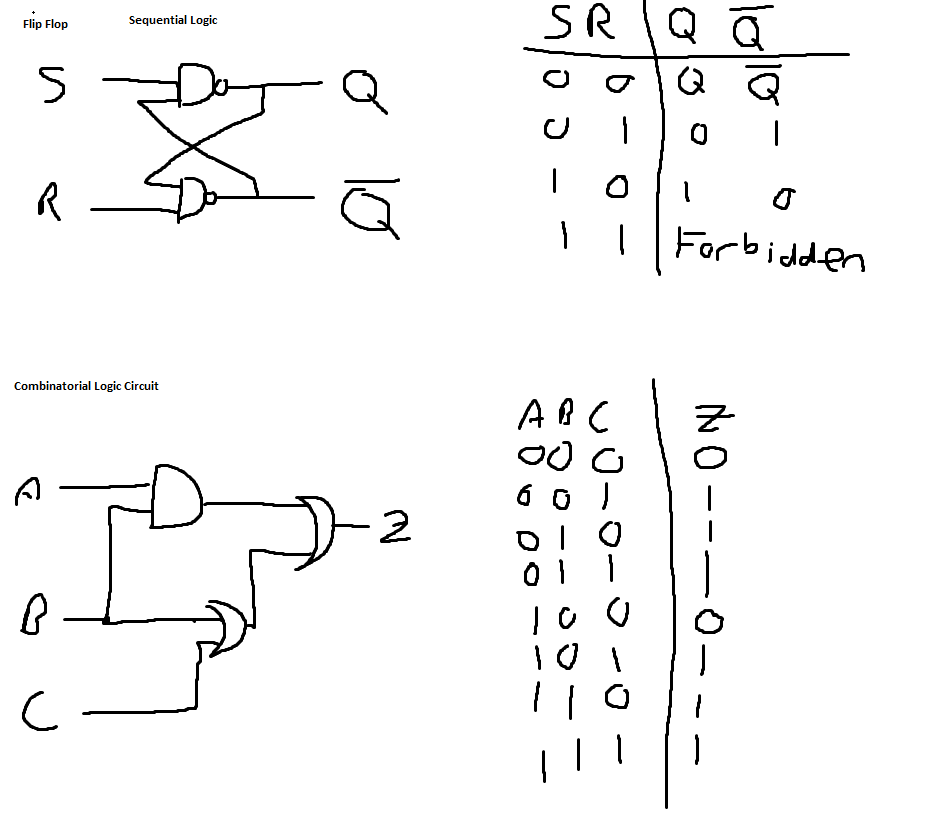
\includegraphics[width=100mm]{digitalLogic.PNG}
    \caption{examples}
    \label{fig:my_label}
\end{figure}

\subsection{Show the truth table for an OR gate.}
\begin{table}[h]
    \centering
    \begin{tabular}{|c|c|c|}
        A & B & Output \\
        0 & 0 & 0\\
        0 & 1 & 1\\
        1 & 0 & 1\\
        1 & 1 & 1\\
    \end{tabular}
    \caption{OR}
    \label{tab:my_label}
\end{table}

\subsection{Show the truth table for an XOR gate.}
\begin{table}[h]
    \centering
    \begin{tabular}{|c|c|c|}
        A & B & Output \\
        0 & 0 & 0\\
        0 & 1 & 1\\
        1 & 0 & 1\\
        1 & 1 & 0\\
    \end{tabular}
    \caption{XOR}
    \label{tab:my_label}
\end{table}

\subsection{Design a circuit that implements the function of an EX-OR gate using only NOT, AND and OR gates.}

\begin{figure}[h]
    \centering
    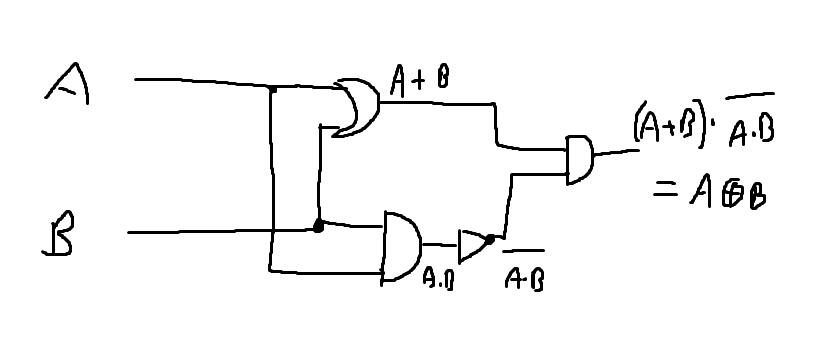
\includegraphics[width=100mm]{digitalLogic2.PNG}
    \caption{examples}
    \label{fig:my_label}
\end{figure}
\newpage
\subsection{Show the truth tables for a AND gate.}
\begin{table}[h]
    \centering
    \begin{tabular}{|c|c|c|}
        A & B & Output \\
        0 & 0 & 0\\
        0 & 1 & 0\\
        1 & 0 & 0\\
        1 & 1 & 1\\
    \end{tabular}
    \caption{AND}
    \label{tab:my_label}
\end{table}

\subsection{Design a circuit that implements the function of an OR gate using only NAND gates.}
\begin{figure}[h]
    \centering
    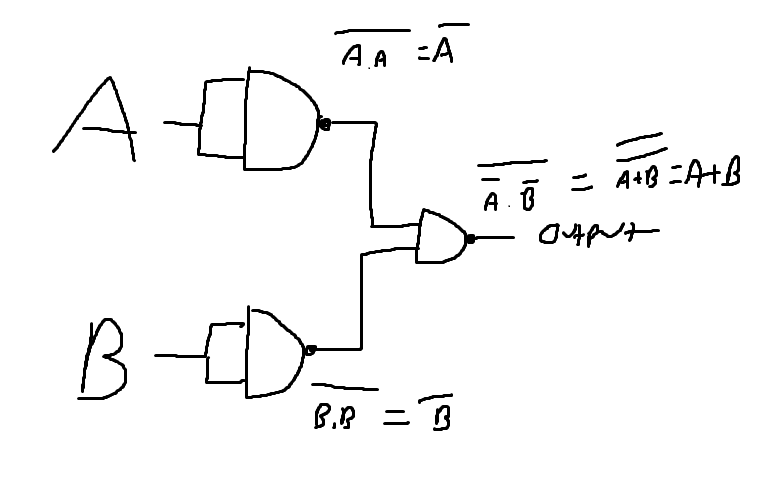
\includegraphics[width=100mm]{digitalLogic3.PNG}
    \caption{examples}
    \label{fig:my_label}
\end{figure}
\newpage
\subsection{Show the truth table for a 1-bit full adder.}
\begin{table}[h]
    \centering
    \begin{tabular}{|c|c|c|c|c|c|}
        A & B & Carry In & & Sum & Carry Out \\
        0 & 0 & 0 & & 0 & 0\\
        0 & 1 & 0 & & 1 & 0\\
        1 & 0 & 0 & & 1 & 0\\
        1 & 1 & 0 & & 0 & 1\\
        0 & 0 & 1 & & 1 & 0\\
        0 & 1 & 1 & & 0 & 1\\
        1 & 0 & 1 & & 0 & 1\\
        1 & 1 & 1 & & 1 & 1
    \end{tabular}
    \caption{1-bit full adder truth table}
    \label{tab:my_label}
\end{table}

\subsection{Design am N-bit Full Adder circuit.}
\begin{figure}[h]
    \centering
    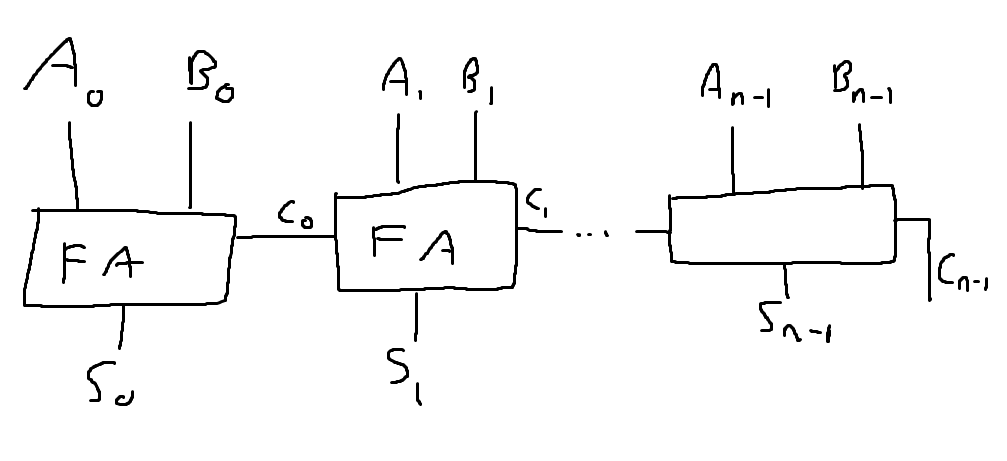
\includegraphics[width=100mm]{digitalLogic4.PNG}
    \caption{examples}
    \label{fig:my_label}
\end{figure}

\subsection{Explain how an N-bit Full Adder circuit can be modified to form an N-bit subtractor circuit.}
We can use the fact that a-b = a+(-b) and have a mode control line (z) that can turn b into -b.\\\\
This can be done by flipping the bits of b and then adding 1. So we can XOR each B in b with the control line. When z is high the bits will be flipped, otherwise they will remain the same. Then to add the extra bit we can just use z as the Carry In to the first 1-bit full adder.
\newpage
\subsection{Design an N-bit Subtractor circuit.}
\begin{figure}[h]
    \centering
    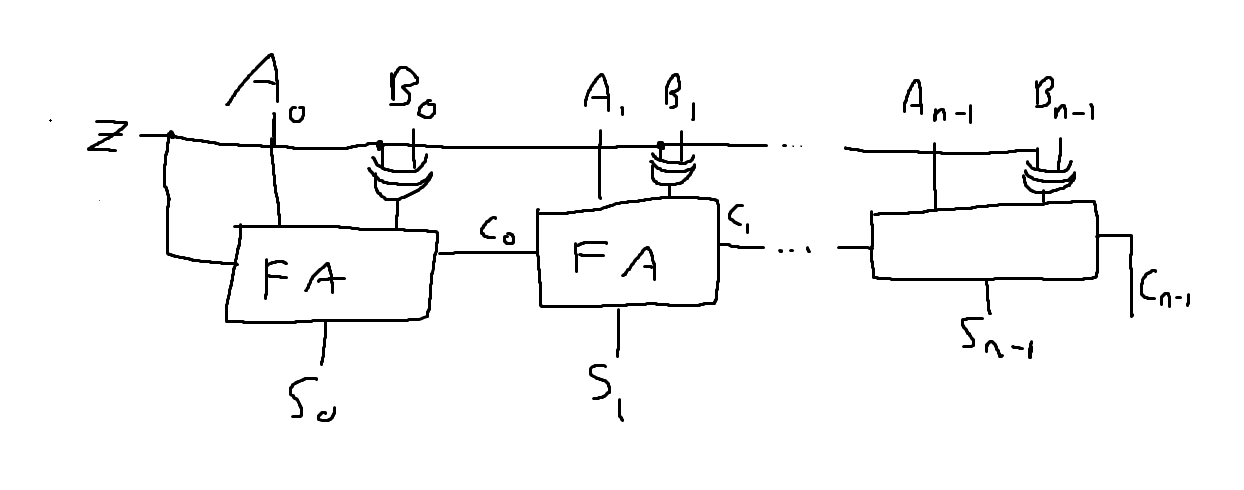
\includegraphics[width=100mm]{digitalLogic5.PNG}
    \caption{examples}
    \label{fig:my_label}
\end{figure}

\subsection{Explain the function of a decoder, giving an example of where a decoder might be used.}
A decoder turns n inputs into $2^n$ outputs. A decoder turns one of the outputs on determined by the binary value of the input.\\
e.g. for an active-low decoder the truth table will be as follows:\\
\begin{table}[h]
    \centering
    \begin{tabular}{|c c|c c c c|}
        $x_0$ & $x_1$ & $y_0$ & $y_1$ & $y_2$ & $y_3$ \\
        0 & 0 & 1 & 0 & 0 & 0\\
        0 & 1 & 0 & 1 & 0 & 0\\
        1 & 0 & 0 & 0 & 1 & 0\\
        1 & 1 & 0 & 0 & 0 & 1
    \end{tabular}
    \caption{decoder}
    \label{tab:my_label}
\end{table}

Decoders are often used to address unique memory locations in a microprocessor system
\newpage
\subsection{Explain the function of a multiplexer, giving an example of where a multiplexer might be used.}
A multiplexer turns n inputs into 1 output, determined by some control modes. A multiplexer turns the output into one of the inputs determined by the control modes.\\
multiplexer truth table for a 4-1 multiplexor (inputs are $x_0, x_1, x_2, x_3$ and control signals are $S_0, S_1$):\\
\begin{table}[h]
    \centering
    \begin{tabular}{|c c|c|}
        $S_0$ & $S_1$ & output\\
        0 & 0 & $x_0$\\
        0 & 1 & $x_1$\\
        1 & 0 & $x_2$\\
        1 & 1 & $x_3$
    \end{tabular}
    \caption{multiplexer}
    \label{tab:my_label}
\end{table}

multiplexers are used for source selection control e.g. home stereo control.

\subsection{Explain, using an appropriate truth table or circuit diagram, the operation of a D-Type latch.}
A D-Type latch is essentially 1 bit of memory. Depending on the current state of the D-Type latch the input to the d-type latch will alter the output.\\
Below is the circuit diagram of a D-Type Latch
\begin{figure}[h]
    \centering
    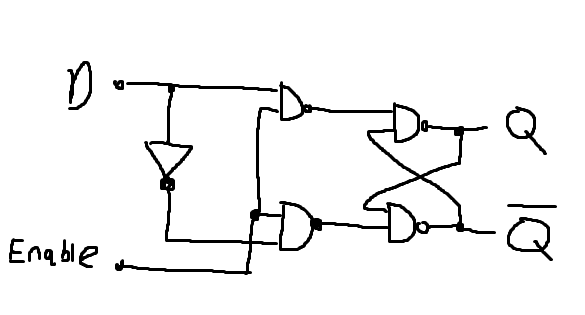
\includegraphics[width=100mm]{digitalLogic6.PNG}
    \caption{d-type latch}
    \label{fig:my_label}
\end{figure}

Below is the truth table for the d-type latch:\newpage
\begin{table}[h]
    \centering
    \begin{tabular}{|c c|c c|}
        Enable & D & Q & $\overline{Q}$\\
        \hline
        0 & 0 & Q & $\overline{Q}$\\
        0 & 1 & Q & $\overline{Q}$\\
        1 & 0 & 0 & 1\\
        1 & 1 & 1 & 0
    \end{tabular}
    \caption{D-Type latch}
    \label{tab:my_label}
\end{table}

\subsection{Show how D-type latches can be arranged to form an N-bit register, explaining the function of your circuit.}
\begin{figure}[h]
    \centering
    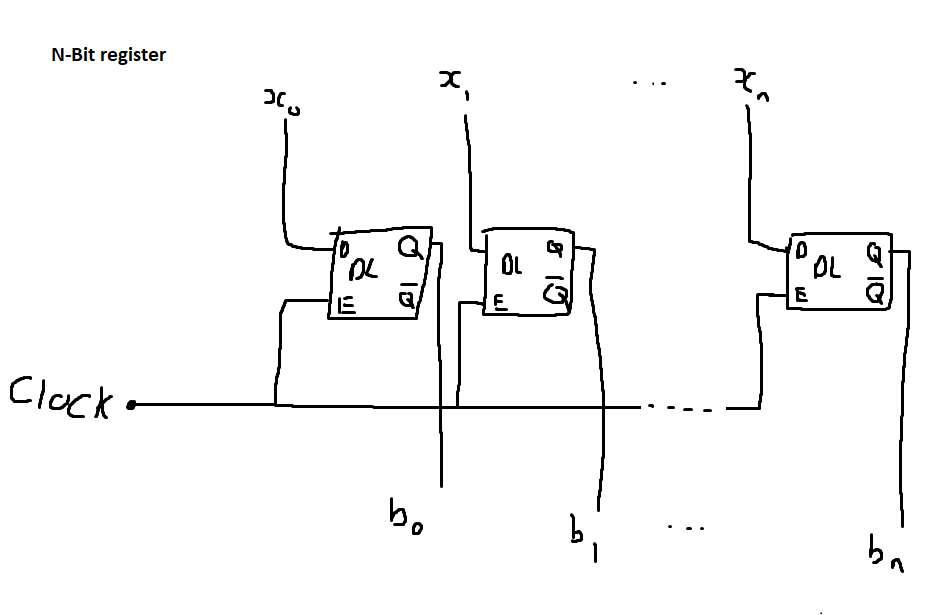
\includegraphics[width=100mm]{digitalLogic7.PNG}
    \caption{d-type latch}
    \label{fig:my_label}
\end{figure}

make note this diagram assumes the D-type latches are rising edge triggered.

\newpage
\section{Assembler quiz (Edmund Goodman)}

\subsection{Explain the role of the Arithmetic Logic Unit (ALU) in the
operations of a microprocessor}

The Arithmetic Logic Unit is a subcomponent of the microprocessor which
performs mathematical and logical operations on data within the
microprocessor.

It is capable of performing various different operation, which can be
selected between by control lines, and is distinct from other components
which read and write the data to provide its inputs and store its
outputs, only handling performing the operations on the data



\subsection{Explain the role of the Control Unit (CU) in the operation
of a microprocessor}

The control unit is a subcomponent of the microprocessor decodes program
instructions into a set of signals which cause and control the logistics
for the execution of the instruction. For example, some signals it
outputs are

It operates at the clock speed of the processor, and is dependent on the
state of other items in the microprocessor (e.g. the CCR)



\subsection{Outline the Fetch-Execute cycle, making reference to the
role it plays in the execution of computer programs}

The fetch-execute cycle is the sequence of steps taken by the computer
to enact a single instruction of machine code (essentially one line of
assembly) stored in memory. These steps are:

\begin{enumerate}
\item
  Fetch
  \begin{enumerate}
  \item
    Retrieve the instruction the main store (MS) at the address
    currently in the program counter (PC)
  \item
    Store the retrieved instruction in the instruction register (IR)
  \item
    Increment the program counter (PC)
  \end{enumerate}
\item
  Decode
  \begin{enumerate}
  \item
    The control unit extracts and decodes the opcode from the
    instruction in the instruction register (IR)
  \item
    Read the effective address to establish opcode type, determining
    whether another read operation is needed
  \end{enumerate}
\item
  Execute
  \begin{enumerate}
  \item
    Control unit outputs signals to control the logistics of executing
    the instruction
  \item
    Changes in the state resulting from the execution of the instruction
    may occur
  \end{enumerate}
\end{enumerate}

Computer programs, irrespective of what language they are written in,
are reduced down to a large sequence of these instructions to be run in
sequence, so the fetch-execute cycle is run many times, once for each
instruction, to execute the program



\subsection{Explain the role of Program Counter (PC) and Instruction
Register (IR) in the Fetch-Execute cycle}

The program counter is use to keep track of which instruction is next to
be executed in the fetch-execute cycle, ensuring the instructions are
evaluated in the correct order. In every cycle, it is incremented after
the instruction is fetched, so it points to the address of the
instruction to be fetched in the next cycle. It can also be moved by
jump instructions, to allow control flow.

The instruction register stores the instruction after it is read from
the location in the main store indicated by the program counter. This
copying is important, as it means it can be accessed quickly, instead of
slower operations of reading the main store, and that in indirect
addressing, it is not overwritten by the data retrieved that is needed
to perform the instruction



\subsection{Explain the purpose of the Condition Code Register (CCR),
giving an example of a situation in which it is used}

The condition control register is a subset of the status register within
the microprocessor, specifically those relating to the condition of the
arithmetic logic unit after the execution of an operation.

One of the ways it may be used is to indicate to the control unit that
an overflow has occurred in an arithmetic operation on two data values



\subsection{With the aid of a diagram, explain the role of a Compiler in
process by which machine code is generated from a high-level computer
program}

The compiler takes program code written in a high level language, such
as C or Rust, and translates it into a sequence of low-level assembly
instructions. Then, an assembler is used to convert these instructions
into machine code. Whilst it does not fully convert between program code
and machine code, it performs the majority of the translation, as
assembly has mostly a one-to-one mapping with machine code

\begin{figure}
\centering
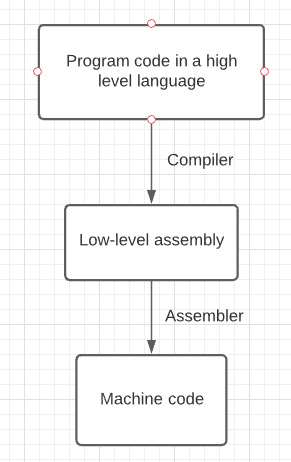
\includegraphics{compilerDiagram.png}
\caption{Compiler diagram}
\end{figure}



\subsection{Show the general form of a statement in assembler, giving a
example of a specific statement and showing how it related to this
general form}

The general form of an instruction is as follows:

\begin{verbatim}
<opcode> <address_1> <address_2> | Comment (optional) 
\end{verbatim}

The opcode indicates what the instruction does, the addresses indicate
what the instruction should be performed on, and the optional comment
indicates what the instruction is being used for

A specific instruction, with the opcode indicating adding, and the
registers being D0 and D1 might be:

\begin{verbatim}
add.l D0, D1 | Add the value of the D1 register to the D0 register
\end{verbatim}



\subsection{Give an example of an arithmetic instruction in assembler
\emph{(not entirely sure if this is correct)}}
\begin{verbatim}
add.l D0, D1 | Add the value of the D1 register to the D0 register
\end{verbatim}
Using direct addressing on a long word, add the value of the D1 register
to the D0 register



\subsection{Explain immediate addressing, giving an example of an
instruction that uses this addressing mode}

Immediate addressing is when the actual value to be used is stored as a
fixed value within the instruction. For example, an instruction to
always add a constant number to a register might be as follows:

\begin{verbatim}
add.l D0,#$42 | Add the hexadecimal value 42 to the register D0
\end{verbatim}



\subsection{Explain absolute addressing, giving an example of an
instruction that uses this addressing mode and showing one disadvantage
of absolute addressing}

Absolute addressing is when the actual address of the value to retrieve
from the main store memory is stored as a fixed value within the
instruction. For example, an instruction to always add the value stored
at a fixed address to a register might be as follows:

\begin{verbatim}
add.l D0, $FFF00 | Add the value at the address FFF00 in the
                   main store to the register D0
\end{verbatim}

This has the disadvantage of the fact the most programs are placed in
different places in memory at each run-time, dependent on what other
programs the computer is performing at the same time. Hence, absolute
addressing is unlikely to point to data within the remit of the program,
so is not useful


\newpage
\section{Memory systems quiz (Edmund Goodman)}

\subsection{Give four factors that influence the selection of an
appropriate memory technology}

\begin{enumerate}
\item
  Cost of production
\item
  Access speed
\item
  Frequency of access
\item
  Capacity
\end{enumerate}


\subsection{Explain the ``designer's dilemma'' for memory systems}

The designers dilemma is the trade-off in designing memory which is
fast, high capacity, and cheap to manufacture. It is not possible to
design memory which achieves all of the properties, so the dilemma is
how to select which ones to best fit the use case


\subsection{Explain, using a diagram, the memory hierarchy}

The memory hierarchy is a way of approaching the designers dilemma to
get the best of each of the properties.

Small amounts of very fast, frequently accessed memory close to the
microprocess (registers and cache) are used to allow the computer to
perform operations very quickly, without having all of the memory of
this type, as that would limit capacity and cost a huge amount.

Further away from the microprocessor, slower, higher capacity and
cheaper memory is used to store data which is less commonly accessed, so
high speeds are not needed.

The diagram below shows a representation of the memory hierarchy:

\begin{figure}
\centering
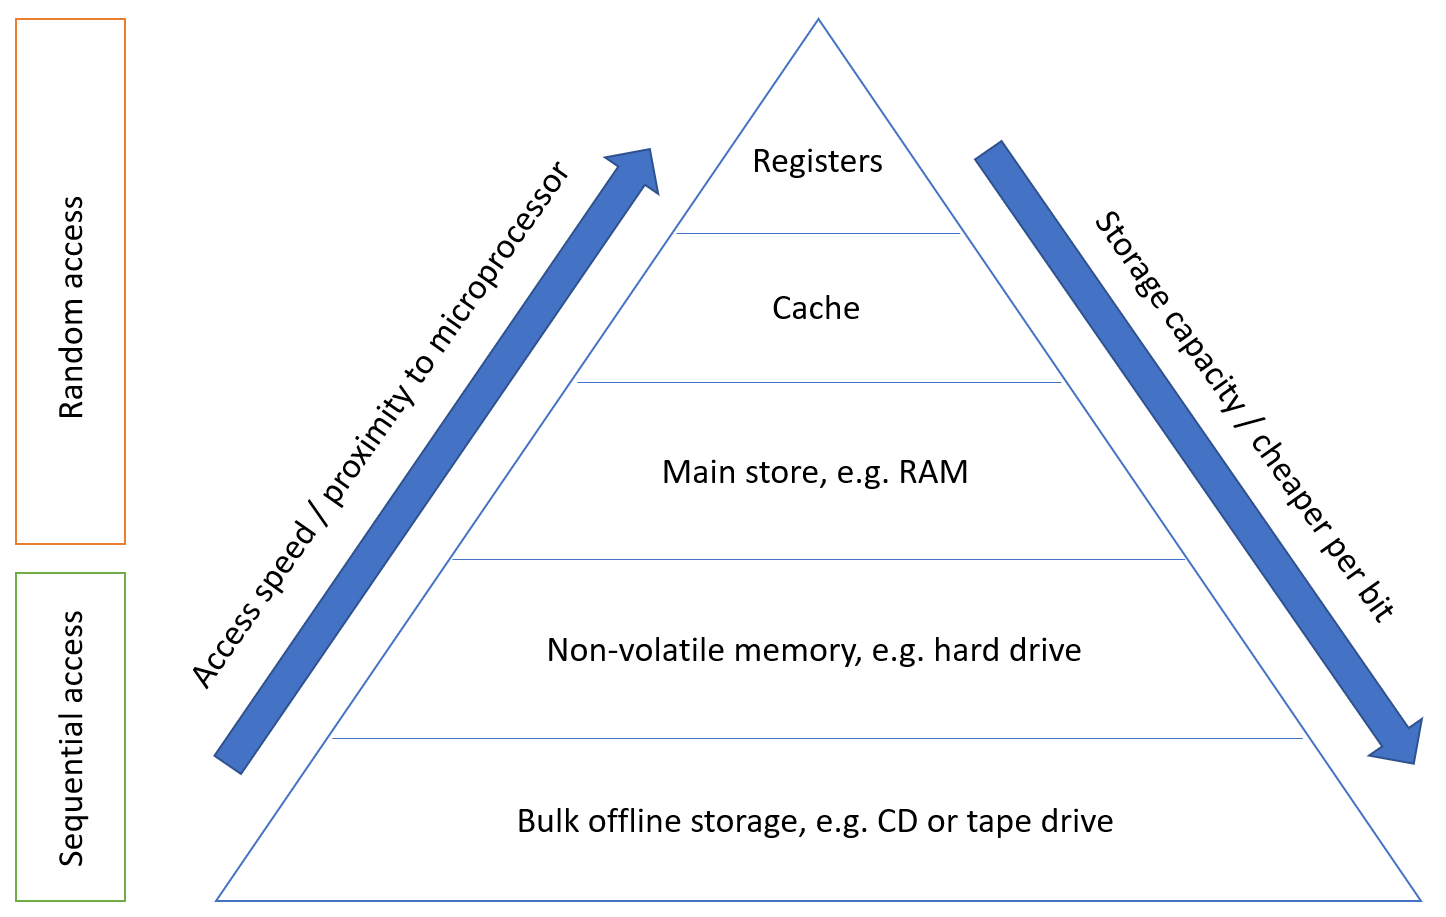
\includegraphics[width=\textwidth]{./memoryHeirarchy.png}
\caption{The memory heirarchy}
\end{figure}


\subsection{Explain the role of cache memory}

Cache memory is a small amount (typically tens of kilobytes) of memory
near the microprocessor which can be accessed very quickly. Cache memory
can be used to store values in memory which are likely to be retrieved,
so the read times are quicker than out of the main store

In computer systems, the next memory location to be accessed is very
likely to be close to the previous memory location accessed. Cache
memory often copies the memory locations around the last memory
location, which means that a significant amount of the time, the cache
already has the memory needed, increasing read speeds


\subsection{How can cache memory exploit spatial locality}

Spatial locality is the idea that memory adjacent to the program counter
position is much more likely to be accessed next than other memory in
the computer (estimates say that 90\% is within 2 kilobytes to either
side). This means that the cache can store this memory, allowing faster
access then if it had to look it up in the main store


\subsection{How can cache memory exploit temporal locality}

Temporal locality is the idea that some memory is more likely to be used
in the future. If an estimate of what this likely memory is can be made,
it can be stored in the cache, allowing faster access then if it had to
look it up in the main store


\subsection{Explain, using a worked example, how a parity bit can be
used to detect errors. You should state the types of error that your
scheme is capable of detecting and correcting}

A parity bit is an additional bit of information included with data to
be sent used to detect errors that occur in its transmission.

There are two types of parity, odd and even parity. In even parity, the
additional parity bit is used to make the number of the number of ones
and the number of zeroes in a transmission both even. For example, in
8-bit parity, if the 7-bit message: ``0101001'' is sent, then
even-parity would add the parity but ``1'' to the end to make the
message ``''0101001 1'', so the number of zeros and the number of ones
are both even. In odd parity, the same process is applied, but the digit
is added to make both numbers odd.

This error checking scheme can detect when an odd number of bits in the
transmission have been changed (when an even number are changed, it
presents as correct, even though bits have been flipped). This means
that whilst it is robust against single errors, bursts of errors make it
only around 50\% effective.

There is no way to identify where the error occurred, so if an error is
detected, it is corrected by replying to the sender that a
re-transmission is needed


\subsection{Explain, using a worked example, how error correcting codes
can use bit- and column-parity to detect and correct errors. You should
state the types of error that your scheme is capable of detecting and
correcting}

Bit and column parity extends using single parity bits, by not only
having a parity bit at the end of each ``word'', e.g. a byte with 7 bits
of message and one of parity, but also sending a parity ``word'' after a
group of words in the same way of a parity bit after a group of message
bits.

For example, in even parity:

\begin{quote}
0101010 1
0110011 0
0111000 1
0110100 1
0101000 0
0111100 0
0000011 0
\end{quote}

The parity word at the end is a parity bit of the column - for example,
the first column is 0000000, so the parity bit would be another 0. In
this example, the parity word is 0000010, with each being the parity bit
of the column.

All burst errors, up to 14 bits can be identified using this schema, and
they can be corrected by looking up the failed parity bit by which row
and which column had incorrect bits, and flipping them











\newpage
\section{I/O Mechanisms Test (Josh Fitzmaurice)}
\subsection{Explain Memory-mapped IO}
Memory mapped I/O is where Memory on IO devices are given address values that a CPU can access.\\
These address locations can be accessed using the same address bus as used for memory.\\
--need one more point

\subsection{Discuss the advantages and disadvantages of memory-mapping as a mechanism for I/O}
Advantages:\\
Memory-mapped IO is simpler than many alternatives and there requires less internal logic which can make the design and fabrication of a CPU cheaper.\\
Disadvantages:\\
Portions of memory must be reserved for IO.\\
For 16-bit and 32-bit systems this becomes a problem as there are not as many address spaces available.

\subsection{Explain the concept of Polling}
Polling is where we check whether the IO device is ready to be used. If it is not ready we go back and read the status, or we could interleave another task to be done while waiting for the status to be ready.\\
\begin{figure}[h]
    \centering
    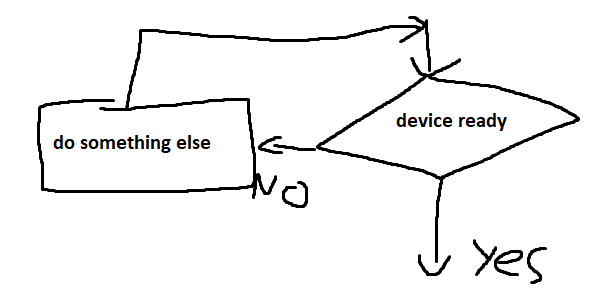
\includegraphics[width = 80mm]{IO.PNG}
    \caption{Polling}
    \label{fig:my_label}
\end{figure}
\newpage

\subsection{Contrast busy-wait and interleaved polling. Your answer should use labelled diagrams where appropriate.}
busy-wait polling is where we read the status of an IO device and if it is not ready we just read the status again on repeat until its ready.

\begin{figure}[h]
    \centering
    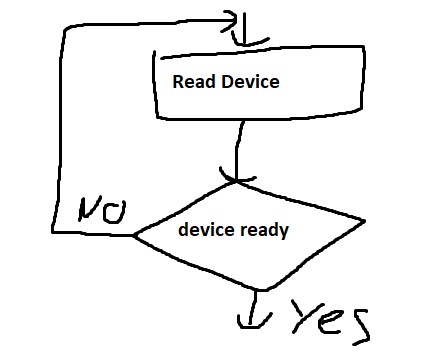
\includegraphics[width = 80mm]{IO3.PNG}
    \caption{busy-wait polling}
    \label{fig:my_label}
\end{figure}

Interleaved polling is similar but instead of just repeatedly checking whether the device is ready, we do another task while waiting for the device to be ready. This allows for better multi-tasking.
\begin{figure}[h]
    \centering
    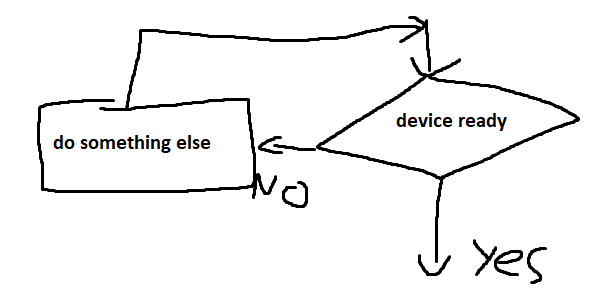
\includegraphics[width = 80mm]{IO.PNG}
    \caption{interleaved polling}
    \label{fig:my_label}
\end{figure}

\subsection{Discuss the advantages and disadvantages of polling}
advantages:\\
Simple software and hardware required to perform polling. Need a looping construct for software and a notion of "ready" for hardware.\\
disadvantages:\\
A lot of CPU time and power is wasted on checking IO devices.\\
Also, interleaving tasks can lead to a significantly delayed response to a device.

\subsection{Explain, using appropriate diagrams, how interrupts can be used to provide asynchronous IO}
\begin{figure}[h]
    \centering
    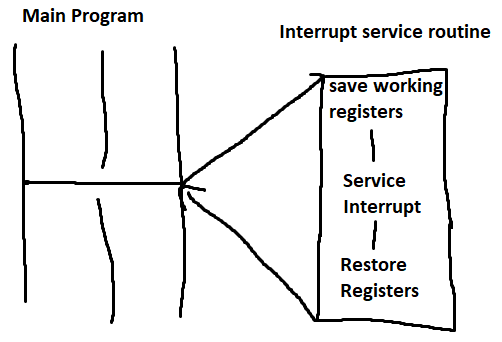
\includegraphics[width = 80mm]{IO2.PNG}
    \caption{Interrupt}
    \label{fig:my_label}
\end{figure}

The figure above shows how when an interrupt is called a Jump is made to a service routines which is performed before going back to the main program.\\
These interrupts forces the CPU to jump between service routines which can make it appear that the CPU is performing 2 or more tasks "simultaneously"

\subsection{Explain context switching}

when an interrupt is called the CPU completes its current instruction then pushes the PC and SR's to a stack.\\
Then load the PC with the address of the Interrupt Handler.\\\\
When returning from an Interrrupt we pop the PC and SR's from the stack then load the PC with the popped return addresses.

\subsection{Discuss the advantages and disadvantages of interrupts as a mechanism for IO}
Advantages:\\
Fast response\\
No wasted CPU time\\\\
Disadvantages:\\
All data trannsfer is controlled by the CPU\\
complex hardware and software.

\subsection{Contrast the suitability of polling and interrupt driven IO for use in an embedded system of your choice. Your answer should state any assumptions clearly}
Chosen embedded system - A safety critical system for an airplane.\\
For a device like this polling would be detrimental as there will be a lot of time where we are checking whether an IO device is ready to respond instead of performing the safety-critical operation. This means that there is a lot of time where the CPU is not performing its operation.\\
Interrupts are much better suited for a safety critical system. This is because a lot less time is wasted on checking whether IO devices are ready to be used. This means there is a fast response which is needed for safety-critical systems

\subsection{Explain Direct Memory Access (DMA). Your answer should give an example of where DMA would be a suitable choice as an I/O mechanism.}

DMA is where the use of system busses is surrendered by the CPU to a DMA Controller (DMAC). This avoids the bottleneck of the CPU for I/O.\\
When an IO device needs to access the system busses they request a DMA transfer, the DMAC passes the request to the CPU. Then the CPU initialises DMAC which requests use of system buses. The CPU then responds with a DMA Ack when it's ready to surrender buses.\\
There are 2 modes of operations for DMA: cycle stealing and Burst Mode.\\
Cycle stealing is where the DMAC uses system busses when they are not being used by the CPU.\\
Burst mode is where the DMAC requires system buses for extended transfer of large amounts of data. The DMAC locks the CPU out of using the system buses for a fixed time or until the CPU received an interrupt from a greater priority.
\newpage




\section{Processor Architecture (Justin Tan)}

\subsection{Distinguish between macro and micro instructions}

Micro instructions are the individual signals that the control unit has to assert to a microprocessor to change the state of values in the processor. When several micro instructions are executed in the right sequence, the microprocessor computes an overall result. \\
This sequence of instructions are specified by a macro instruction in the form of an opcode which is fed into the control unit from the instruction register. The control unit is able to translate this opcode into the appropriate sequence of micro instructions that achieve the desired result mentioned earlier.

\subsection{Relate the fetch-execute cycle to the execution of macro and micro instructions}

Before each macro instruction is received as an opcode, the control unit has to fetch it. The contents of the program counter are passed to the MAR, the MAR sends this to Main store to retrieve the data from the address. This data is typically passed to the MDR and then the IR, and the opcode is then sent to the control unit. \\
This opcode is translated to a sequence of control signals by the control unit, and each of these signals is a micro instruction. When carried out in the right sequence, these micro instructions compute a result which is the desired result of the macro instruction. To execute the next macro instruction, the control unit has to fetch the next set of instructions and then execute it.


\subsection{Give a detailed explanation of the hardwired approach to control unit design}

The hardwired approach consists of 4 main components. The sequencer takes the clock input of our microprocessor, and its main role is to align the operation of the combinatorial logic circuit in the control unit (CU) with the control steps for each macro instruction that depend on the microprocessor's clock. Hence these regulated signals should ideally match the clock frequency. \\
The instruction decoder decodes the opcode and sends a signal down the right path that will have the appropriate logic gates to assert the right signals to other subsystems together with the sequencer. \\
The fetch/execute flip-flop works together with the sequencer to regulate the control rounds, essentially making sure that the sequencer is in sync with the start and end of control rounds.\\
Lastly, the main component in the control unit contains the combinatorial logic circuit that has inputs from the decoder and outputs to communication busses that connect to the rest of the microprocessor. It also has output lines to the flip-flop to signify when certain control rounds start and end.

\subsection{Discuss the advantages and disadvantages of using a hardwired approach to control unit design}

The advantages are that it is very fast, as it operates at the speed of logic gates. \\
The disadvantages are a long design time because of complex hardware, there is no backward compatibility, and it is inflexible as it is difficult to change the design if new instructions are added.

\subsection{Given a detailed explanation of the micro-programmed approach to control unit design}

The CU with this approach is made up of a few components. Firstly there is an OTOA circuit, which is essentially a lookup table that translates opcodes into microprogram addresses. \\
This is fed into a CN circuit that is meant to control the value given to the micro program counter (microPC). The microPC is the internal PC of the CU and it stores the value of the address of the microprogram to be executed next. Before each opcode is received, the microPC will have to point to the starting microaddress of the fetch microprogram that initiates the macro fetch operation in the processor. Otherwise, it points to the microaddress specified by the opcode. \\
The microprogram memory is the internal memory of the CU that stores the microinstructions for each microprogram at its respective microaddress location. \\
It feeds microinstructions based on the microadress to the microIR, which then takes the values in the instruction and sets the appropriate output values for the CU. 
\\
Microinstructions are typically executed in sequence, incremented by the microPC, until the last microinstruction is executed. When this happens the microPC is set such that it either points back to microadress 0 which corresponds to the starting address of the fetch microprogram or points to the microaddress set by the OTOA.

\subsection{Discuss the advantages and disadvantages of using a micro-programmed approach to control unit design}

The advantages are that is easy to design and implement, there is backward compatibility because it is can be reprogrammed for new instructions but still accept older instructions. Its hardware is simple compared to hardwired implementations and its flexibility of design allows families of processors to be built. \\
Its disadvantage is that it is slower than hardwired implementations.

\subsection{Distinguish between CISC and RISC architectures, giving a specific example of each}

CISC architectures primarily use the micro-programmed approach for control unit design, while RISC architectures use a hard-wired approach. A very well known example of RISC is of computer chips made from the company ARM (Advanced RISC Machine). While Intel uses a hybrid approach, commonly used instructions are hardwired, while others are micro-programmed, their chips are a good example of ones that use the CISC architecture.

\end{document}
